\chapter{Reynolds Number Effect on the Centerline Velocity of a Supersonic Jet}
\label{Appendix: Ozawa centerline}

\par Section \ref{subsection: Quantitative Density Field results} compares the centerline density of the compressible jet imaged in this work with the data of Panda and Seasholtz \cite{Panda1999}, whose nozzle diameter is about seven times larger. The difference in Reynolds number that follows from this is argued there to explain why the measurements of this work decay more slowly downstream. The evidence for that argument comes from Ozawa et al. \cite{Ozawa2020}, who measured three supersonic jets at the same Mach number and different Reynolds numbers. Their result is reproduced in Figure \ref{fig: Ozawa centerline velocity} so the reader can judge the comparison directly.

\begin{figure}[htbp]
    \centering
    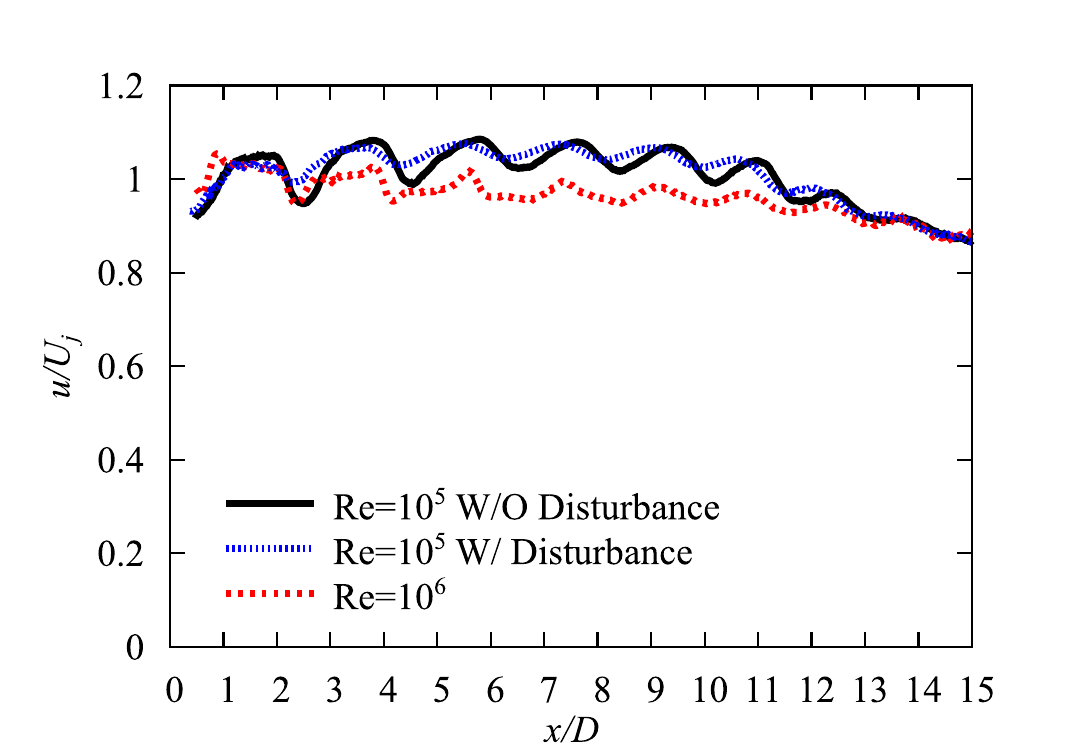
\includegraphics[width=0.75\textwidth]{figures/Ozawa centerline velocity.png}
    \caption[Centerline velocity of supersonic jets at two Reynolds numbers]{Streamwise distribution of the axial velocity along the centerline of three supersonic jets, measured with particle image velocimetry. The black and blue curves are the low Reynolds number jet, $Re = 10^5$, without and with a disturbance added at the nozzle inlet, and the red curve is the high Reynolds number jet, $Re = 10^6$. Reproduced from Figure 12 of Ozawa et al. \cite{Ozawa2020}}
    \label{fig: Ozawa centerline velocity}
\end{figure}

\par Two features of the figure support the interpretation given in Chapter \ref{chapter: Results}. First, the red curve of the high Reynolds number jet sits below the two low Reynolds number curves from about $x/d_N = 3$ to $x/d_N = 12$, which shows that the centerline velocity decays faster when the Reynolds number is higher. Second, the oscillations produced by the shock cells are weaker and less regular in the red curve, while the low Reynolds number jets hold a clear periodic structure over the whole range.

\par The same work places the transition at $Re \approx 10^5$, which it describes as a transitional condition between a partially laminar and a fully turbulent shear layer, and reports that the Reynolds number ceases to affect the turbulent features above $Re \approx 4 \cdot 10^5$. The jet imaged in this work sits at $Re = 1.78 \cdot 10^5$ and that of Panda and Seasholtz at $Re = 1.29 \cdot 10^6$, so the two fall on opposite sides of that boundary.
